\large{
سیستم‌های مبتنی بر مدل‌سازی رابطه‌ای که توسط Codd ارائه شده بود؛ که به عنوان مدل جدولی هم شناخته . این یک مفهوم فرافایلی است. 
}

\\

\textbf{
تعریف پایگاه داده: مجموعه‌ای است از داده‌های ذخیره شده، پایا، محتمع، به هم مرتبط، و حتی الامکان فاقد افزونگی، (دارای معماری خاص خود، مبتنی بر یک مدل داده ای مشخص)،  تحت کنترل یک سیستم متمرکز، مورد استفاده یک یا چند کاربر، در یک سازمان (در یک محیط)، به طور اشتراکی و همروند.
}

\large{تاریخجه سیستم‌های ذخیره سازی و بازیابی اطلاعات}

\graphicspath{ {./files/} }


 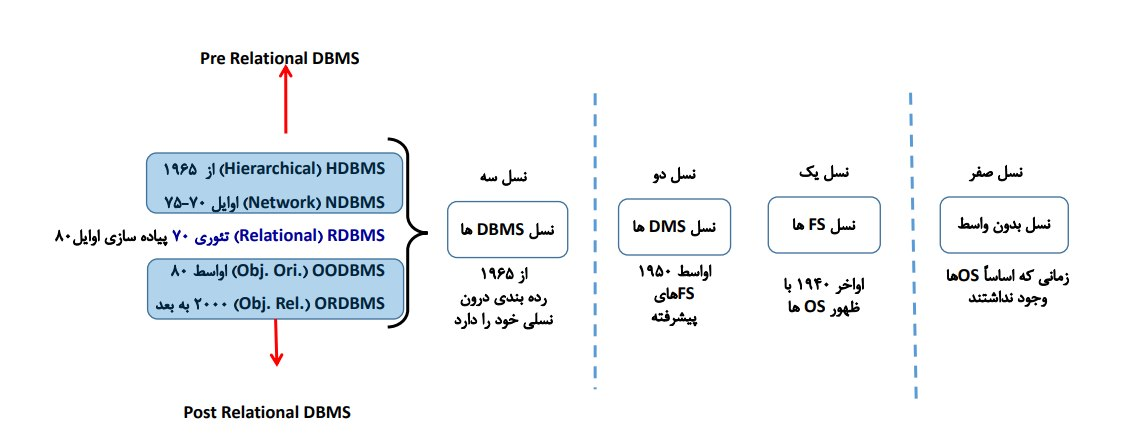
\includegraphics[scale=0.5]{1}


\large{
یادداشت: OODBSها در واقع تلاشی (ناموفق) بودند برای اینکه ایده‌های شیء گرا را در database ها پیاده کنند.
}

